\chapter{Software Defined Networking}

SDN is often referred to as a ``radical new idea of networking''. It has been made to overcome many requirements and current network technology limitations which arose in the last years:
\begin{enumerate}
   \item[] \ul{The demand is increasing}
   \item Cloud computing
   \item Big Data
   \item Mobile traffic
   \item IoT
   \item[] \ul{\textit{Supply} also increasing}
   \item Network technologies capable of absorbing high load
   \item Performance of network devices increased
   \begin{enumerate}
      \item CPU speed
      \item Buffer capacity and speed
      \item etc...
   \end{enumerate}
   \item[] \ul{\textit{Traffic patterns}\footnote{Traffic patterns measure how traffic varies in time and space} have changed and became more dynamic and complex} 
   \note{This is the most critical aspect}
\end{enumerate}

\section{Traffic Patterns}
Modern distributed applications typically access multiple databases and servers that
must communicate with each other, creating a lot of
\textit{``horizontal''} traffic between servers ---in addition to the \textit{``vertical''} client/server one--- which was initially neglectable, but now it is not.

Unified communications (UC) services are increasingly used within enterprises. Many communication services such as instant messaging (chat), presence
information, voice, mobility, audio, web and video traffic, must be \textit{integrated} into a unique service
delivery platform

TODO

\section{Layering}
Layering, as it is applied in TCP/IP stack, implies decomposing delivery into fundamental components, allowing independent but compatible innovation at each layer; it revealed itself to be pretty successful, however, \ul{many issues reside in the \textit{Network Control/Management Plane}}.

If in computer science usually many clean and elegant abstractions are used, network control instead is strongly related to hardware and verbose protocols, there are \textit{no} principles or abstractions guiding the process, making in general difficult managing traffic flows.

SDN helps providing some abstraction through a centralized view of the network.

\subsection{Network Layer}
\begin{itemize}
   \item \textbf{Forwarding} move packets from router’s input to appropriate router output
   \note{Data Plane}
   \item \textbf{Routing} determine route taken by packets from
   source to destination
   \note{Control Plane}
\end{itemize}

These are the two key tasks. In Fig. a comparison between the tradional and the SDN approaches.
\begin{figure}[htbp]
   \centering
   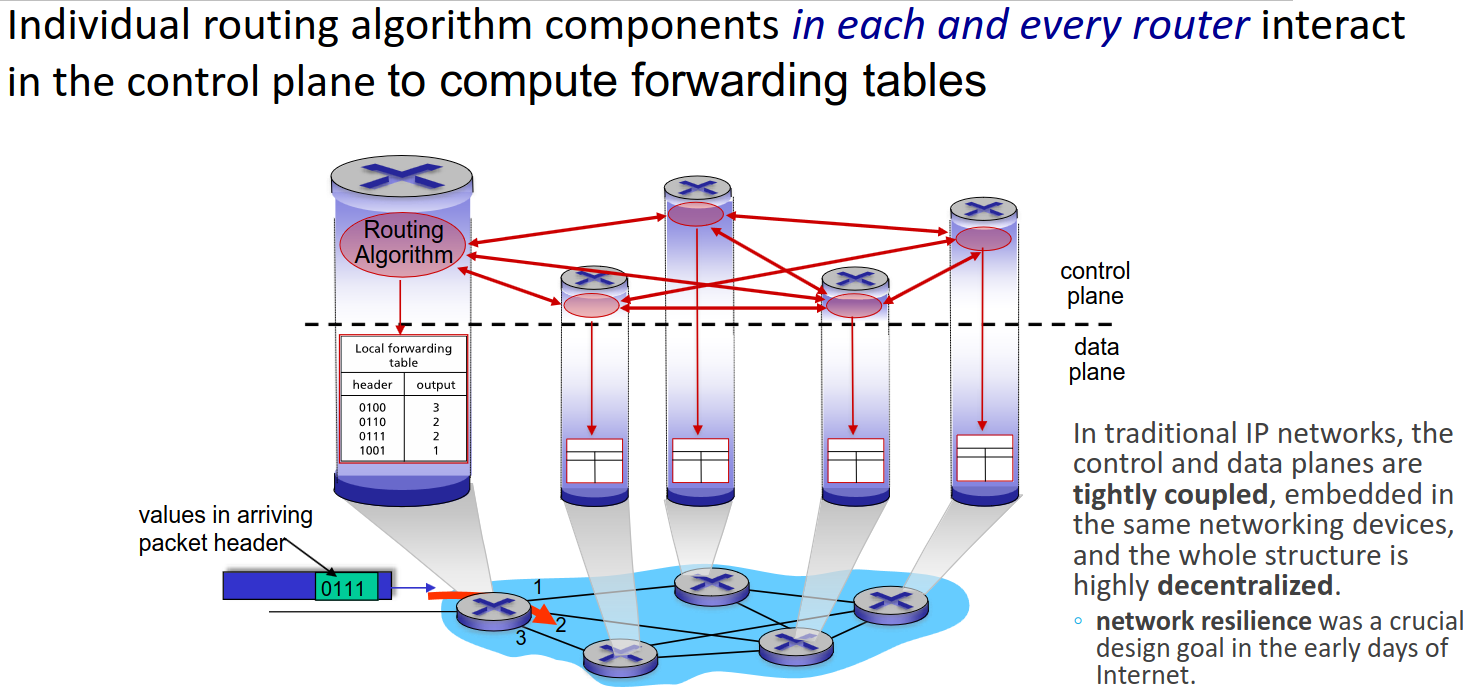
\includegraphics[width=0.45\columnwidth]{images/sdn_planes1.png}
   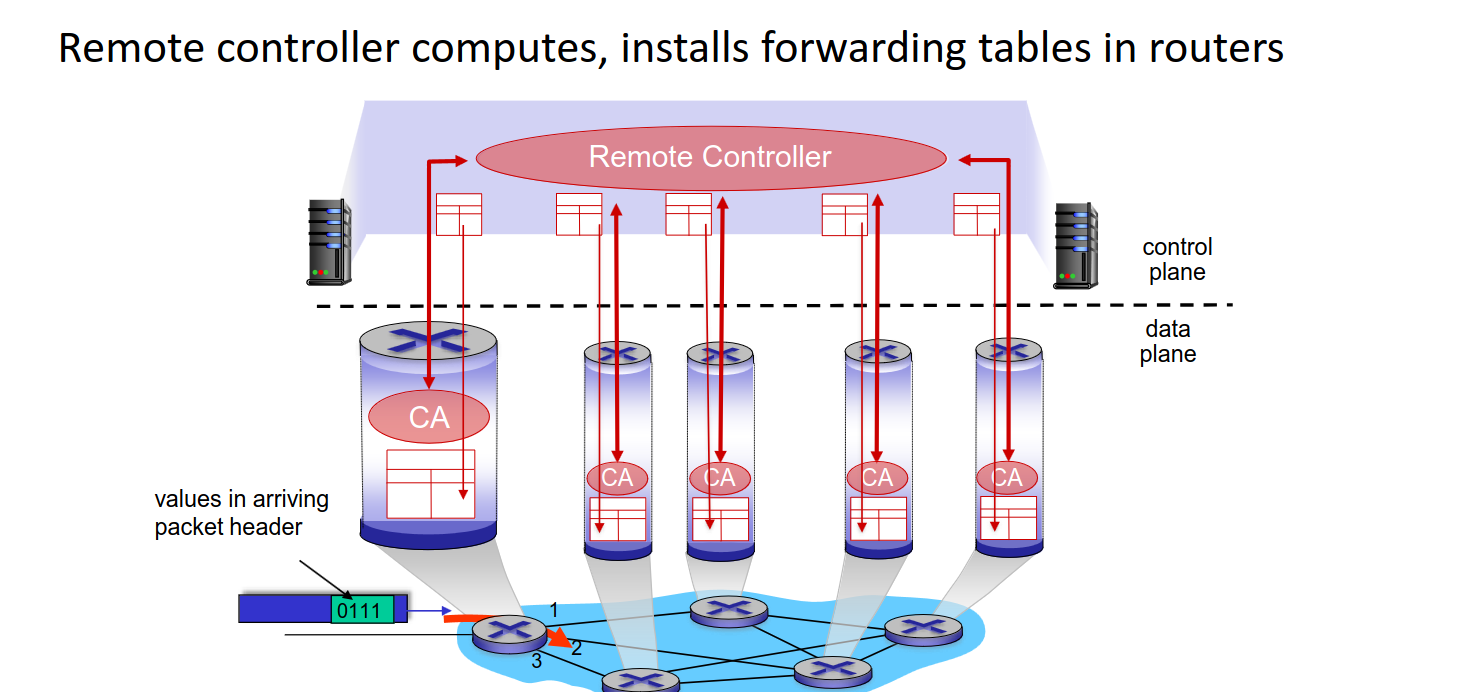
\includegraphics[width=0.45\columnwidth]{images/sdn_planes2.png}
   \caption{Traditional vs SDN}
   \label{fig:sdn_planes}
\end{figure}

\begin{paracol}{2}
   \textbf{Data-plane switches} are fast, simple, commodity switches implementing generalized data-plane forwarding in hardware, and generally provide API for table-based switch control, e.g. \texttt{OpenFlow}.

   \textbf{SDN controller} (network OS) maintain network state information and interacts with network control applications ``above'' via northbound API, and with switches using ``below'' via southbound API.
   They are implemented as distributed system for performance, scalability, fault-tolerance, robustness.

   \textbf{Network-control apps} are ``brains'' of control, they implement control functions using lower-level services. They are \textit{unbundled}, meaning that they may be provided by a $3^{rd}$ party different from routing vendor or SDN controller
   \switchcolumn
   \begin{figure}[htbp]
      \centering
      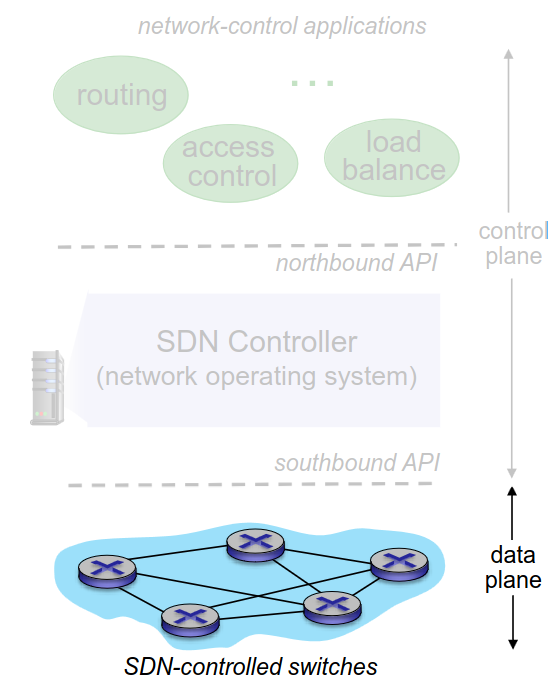
\includegraphics{images/sdn_planes3.png}
      \caption{SDN Layer Architectures}
      \label{fig:sdn_planes3}
   \end{figure}
\end{paracol}